\documentclass[1p]{elsarticle_modified}
%\bibliographystyle{elsarticle-num}

%\usepackage[colorlinks]{hyperref}
%\usepackage{abbrmath_seonhwa} %\Abb, \Ascr, \Acal ,\Abf, \Afrak
\usepackage{amsfonts}
\usepackage{amssymb}
\usepackage{amsmath}
\usepackage{amsthm}
\usepackage{scalefnt}
\usepackage{amsbsy}
\usepackage{kotex}
\usepackage{caption}
\usepackage{subfig}
\usepackage{color}
\usepackage{graphicx}
\usepackage{xcolor} %% white, black, red, green, blue, cyan, magenta, yellow
\usepackage{float}
\usepackage{setspace}
\usepackage{hyperref}

\usepackage{tikz}
\usetikzlibrary{arrows}

\usepackage{multirow}
\usepackage{array} % fixed length table
\usepackage{hhline}

%%%%%%%%%%%%%%%%%%%%%
\makeatletter
\renewcommand*\env@matrix[1][\arraystretch]{%
	\edef\arraystretch{#1}%
	\hskip -\arraycolsep
	\let\@ifnextchar\new@ifnextchar
	\array{*\c@MaxMatrixCols c}}
\makeatother %https://tex.stackexchange.com/questions/14071/how-can-i-increase-the-line-spacing-in-a-matrix
%%%%%%%%%%%%%%%

\usepackage[normalem]{ulem}

\newcommand{\msout}[1]{\ifmmode\text{\sout{\ensuremath{#1}}}\else\sout{#1}\fi}
%SOURCE: \msout is \stkout macro in https://tex.stackexchange.com/questions/20609/strikeout-in-math-mode

\newcommand{\cancel}[1]{
	\ifmmode
	{\color{red}\msout{#1}}
	\else
	{\color{red}\sout{#1}}
	\fi
}

\newcommand{\add}[1]{
	{\color{blue}\uwave{#1}}
}

\newcommand{\replace}[2]{
	\ifmmode
	{\color{red}\msout{#1}}{\color{blue}\uwave{#2}}
	\else
	{\color{red}\sout{#1}}{\color{blue}\uwave{#2}}
	\fi
}

\newcommand{\Sol}{\mathcal{S}} %segment
\newcommand{\D}{D} %diagram
\newcommand{\A}{\mathcal{A}} %arc


%%%%%%%%%%%%%%%%%%%%%%%%%%%%%5 test

\def\sl{\operatorname{\textup{SL}}(2,\Cbb)}
\def\psl{\operatorname{\textup{PSL}}(2,\Cbb)}
\def\quan{\mkern 1mu \triangleright \mkern 1mu}

\theoremstyle{definition}
\newtheorem{thm}{Theorem}[section]
\newtheorem{prop}[thm]{Proposition}
\newtheorem{lem}[thm]{Lemma}
\newtheorem{ques}[thm]{Question}
\newtheorem{cor}[thm]{Corollary}
\newtheorem{defn}[thm]{Definition}
\newtheorem{exam}[thm]{Example}
\newtheorem{rmk}[thm]{Remark}
\newtheorem{alg}[thm]{Algorithm}

\newcommand{\I}{\sqrt{-1}}
\begin{document}

%\begin{frontmatter}
%
%\title{Boundary parabolic representations of knots up to 8 crossings}
%
%%% Group authors per affiliation:
%\author{Yunhi Cho} 
%\address{Department of Mathematics, University of Seoul, Seoul, Korea}
%\ead{yhcho@uos.ac.kr}
%
%
%\author{Seonhwa Kim} %\fnref{s_kim}}
%\address{Center for Geometry and Physics, Institute for Basic Science, Pohang, 37673, Korea}
%\ead{ryeona17@ibs.re.kr}
%
%\author{Hyuk Kim}
%\address{Department of Mathematical Sciences, Seoul National University, Seoul 08826, Korea}
%\ead{hyukkim@snu.ac.kr}
%
%\author{Seokbeom Yoon}
%\address{Department of Mathematical Sciences, Seoul National University, Seoul, 08826,  Korea}
%\ead{sbyoon15@snu.ac.kr}
%
%\begin{abstract}
%We find all boundary parabolic representation of knots up to 8 crossings.
%
%\end{abstract}
%\begin{keyword}
%    \MSC[2010] 57M25 
%\end{keyword}
%
%\end{frontmatter}

%\linenumbers
%\tableofcontents
%
\newcommand\colored[1]{\textcolor{white}{\rule[-0.35ex]{0.8em}{1.4ex}}\kern-0.8em\color{red} #1}%
%\newcommand\colored[1]{\textcolor{white}{ #1}\kern-2.17ex	\textcolor{white}{ #1}\kern-1.81ex	\textcolor{white}{ #1}\kern-2.15ex\color{red}#1	}

{\Large $\underline{11a_{253}~(K11a_{253})}$}

\setlength{\tabcolsep}{10pt}
\renewcommand{\arraystretch}{1.6}
\vspace{1cm}\begin{tabular}{m{100pt}>{\centering\arraybackslash}m{274pt}}
\multirow{5}{120pt}{
	\centering
	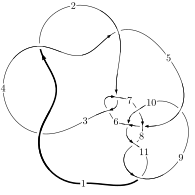
\includegraphics[width=112pt]{../../../GIT/diagram.site/Diagrams/png/502_11a_253.png}\\
\ \ \ A knot diagram\footnotemark}&
\allowdisplaybreaks
\textbf{Linearized knot diagam} \\
\cline{2-2}
 &
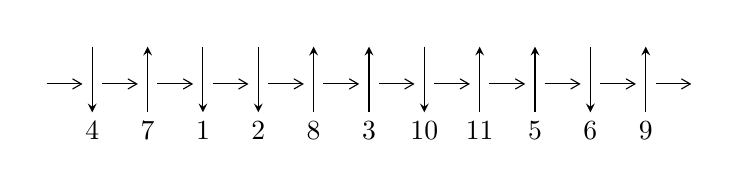
\begin{tikzpicture}[x=20pt, y=17pt]
	% nodes
	\node (C0) at (0, 0) {};
	\node (C1) at (1, 0) {};
	\node (C1U) at (1, +1) {};
	\node (C1D) at (1, -1) {4};

	\node (C2) at (2, 0) {};
	\node (C2U) at (2, +1) {};
	\node (C2D) at (2, -1) {7};

	\node (C3) at (3, 0) {};
	\node (C3U) at (3, +1) {};
	\node (C3D) at (3, -1) {1};

	\node (C4) at (4, 0) {};
	\node (C4U) at (4, +1) {};
	\node (C4D) at (4, -1) {2};

	\node (C5) at (5, 0) {};
	\node (C5U) at (5, +1) {};
	\node (C5D) at (5, -1) {8};

	\node (C6) at (6, 0) {};
	\node (C6U) at (6, +1) {};
	\node (C6D) at (6, -1) {3};

	\node (C7) at (7, 0) {};
	\node (C7U) at (7, +1) {};
	\node (C7D) at (7, -1) {10};

	\node (C8) at (8, 0) {};
	\node (C8U) at (8, +1) {};
	\node (C8D) at (8, -1) {11};

	\node (C9) at (9, 0) {};
	\node (C9U) at (9, +1) {};
	\node (C9D) at (9, -1) {5};

	\node (C10) at (10, 0) {};
	\node (C10U) at (10, +1) {};
	\node (C10D) at (10, -1) {6};

	\node (C11) at (11, 0) {};
	\node (C11U) at (11, +1) {};
	\node (C11D) at (11, -1) {9};
	\node (C12) at (12, 0) {};

	% arrows
	\draw[->,>={angle 60}]
	(C0) edge (C1) (C1) edge (C2) (C2) edge (C3) (C3) edge (C4) (C4) edge (C5) (C5) edge (C6) (C6) edge (C7) (C7) edge (C8) (C8) edge (C9) (C9) edge (C10) (C10) edge (C11) (C11) edge (C12) ;	\draw[->,>=stealth]
	(C1U) edge (C1D) (C2D) edge (C2U) (C3U) edge (C3D) (C4U) edge (C4D) (C5D) edge (C5U) (C6D) edge (C6U) (C7U) edge (C7D) (C8D) edge (C8U) (C9D) edge (C9U) (C10U) edge (C10D) (C11D) edge (C11U) ;
	\end{tikzpicture} \\
\hhline{~~} \\& 
\textbf{Solving Sequence} \\ \cline{2-2} 
 &
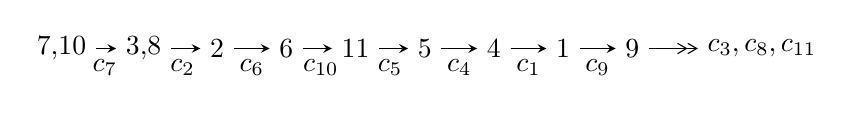
\begin{tikzpicture}[x=25pt, y=7pt]
	% node
	\node (A0) at (-1/8, 0) {7,10};
	\node (A1) at (17/16, 0) {3,8};
	\node (A2) at (17/8, 0) {2};
	\node (A3) at (25/8, 0) {6};
	\node (A4) at (33/8, 0) {11};
	\node (A5) at (41/8, 0) {5};
	\node (A6) at (49/8, 0) {4};
	\node (A7) at (57/8, 0) {1};
	\node (A8) at (65/8, 0) {9};
	\node (C1) at (1/2, -1) {$c_{7}$};
	\node (C2) at (13/8, -1) {$c_{2}$};
	\node (C3) at (21/8, -1) {$c_{6}$};
	\node (C4) at (29/8, -1) {$c_{10}$};
	\node (C5) at (37/8, -1) {$c_{5}$};
	\node (C6) at (45/8, -1) {$c_{4}$};
	\node (C7) at (53/8, -1) {$c_{1}$};
	\node (C8) at (61/8, -1) {$c_{9}$};
	\node (A9) at (10, 0) {$c_{3},c_{8},c_{11}$};

	% edge
	\draw[->,>=stealth]	
	(A0) edge (A1) (A1) edge (A2) (A2) edge (A3) (A3) edge (A4) (A4) edge (A5) (A5) edge (A6) (A6) edge (A7) (A7) edge (A8) ;
	\draw[->>,>={angle 60}]	
	(A8) edge (A9);
\end{tikzpicture} \\ 

\end{tabular} \\

\footnotetext{
The image of knot diagram is generated by the software ``\textbf{Draw programme}" developed by Andrew Bartholomew(\url{http://www.layer8.co.uk/maths/draw/index.htm\#Running-draw}), where we modified some parts for our purpose(\url{https://github.com/CATsTAILs/LinksPainter}).
}\phantom \\ \newline 
\centering \textbf{Ideals for irreducible components\footnotemark of $X_{\text{par}}$} 
 
\begin{align*}
I^u_{1}&=\langle 
-3.29827\times10^{242} u^{70}-3.85213\times10^{243} u^{69}+\cdots+1.61478\times10^{243} b-8.28511\times10^{242},\\
\phantom{I^u_{1}}&\phantom{= \langle  }-1.44895\times10^{243} u^{70}-1.68032\times10^{244} u^{69}+\cdots+1.61478\times10^{243} a+5.61105\times10^{243},\\
\phantom{I^u_{1}}&\phantom{= \langle  }u^{71}+12 u^{70}+\cdots+2 u+1\rangle \\
I^u_{2}&=\langle 
b,\;- u^4- u^3-3 u^2+a- u-2,\;u^5+u^4+2 u^3+u^2+u+1\rangle \\
\\
\end{align*}
\raggedright * 2 irreducible components of $\dim_{\mathbb{C}}=0$, with total 76 representations.\\
\footnotetext{All coefficients of polynomials are rational numbers. But the coefficients are sometimes approximated in decimal forms when there is not enough margin.}
\newpage
\renewcommand{\arraystretch}{1}
\centering \section*{I. $I^u_{1}= \langle -3.30\times10^{242} u^{70}-3.85\times10^{243} u^{69}+\cdots+1.61\times10^{243} b-8.29\times10^{242},\;-1.45\times10^{243} u^{70}-1.68\times10^{244} u^{69}+\cdots+1.61\times10^{243} a+5.61\times10^{243},\;u^{71}+12 u^{70}+\cdots+2 u+1 \rangle$}
\flushleft \textbf{(i) Arc colorings}\\
\begin{tabular}{m{7pt} m{180pt} m{7pt} m{180pt} }
\flushright $a_{7}=$&$\begin{pmatrix}1\\0\end{pmatrix}$ \\
\flushright $a_{10}=$&$\begin{pmatrix}0\\u\end{pmatrix}$ \\
\flushright $a_{3}=$&$\begin{pmatrix}0.897301 u^{70}+10.4058 u^{69}+\cdots-15.1406 u-3.47480\\0.204255 u^{70}+2.38554 u^{69}+\cdots-0.797246 u+0.513078\end{pmatrix}$ \\
\flushright $a_{8}=$&$\begin{pmatrix}1\\u^2\end{pmatrix}$ \\
\flushright $a_{2}=$&$\begin{pmatrix}0.693047 u^{70}+8.02030 u^{69}+\cdots-14.3434 u-3.98788\\0.204255 u^{70}+2.38554 u^{69}+\cdots-0.797246 u+0.513078\end{pmatrix}$ \\
\flushright $a_{6}=$&$\begin{pmatrix}0.991671 u^{70}+11.2338 u^{69}+\cdots-0.635568 u+2.82255\\0.150636 u^{70}+1.87103 u^{69}+\cdots-0.311046 u+0.838335\end{pmatrix}$ \\
\flushright $a_{11}=$&$\begin{pmatrix}-3.05511 u^{70}-38.0827 u^{69}+\cdots-14.2425 u+2.92815\\-0.251356 u^{70}-2.91652 u^{69}+\cdots+4.21504 u+0.652989\end{pmatrix}$ \\
\flushright $a_{5}=$&$\begin{pmatrix}0.976661 u^{70}+11.0121 u^{69}+\cdots+0.0163988 u+2.65051\\0.218015 u^{70}+2.64923 u^{69}+\cdots-0.212886 u+0.879910\end{pmatrix}$ \\
\flushright $a_{4}=$&$\begin{pmatrix}0.0842423 u^{70}+1.02322 u^{69}+\cdots+9.62101 u+4.52032\\-0.0463985 u^{70}-0.516278 u^{69}+\cdots+0.435416 u-0.111771\end{pmatrix}$ \\
\flushright $a_{1}=$&$\begin{pmatrix}0.658958 u^{70}+7.79572 u^{69}+\cdots-9.48146 u-0.610030\\0.0463985 u^{70}+0.516278 u^{69}+\cdots-0.435416 u+0.111771\end{pmatrix}$ \\
\flushright $a_{9}=$&$\begin{pmatrix}-3.25923 u^{70}-40.5525 u^{69}+\cdots-9.10450 u+3.81600\\0.136311 u^{70}+1.50077 u^{69}+\cdots+4.68772 u+1.32234\end{pmatrix}$\\ \flushright $a_{9}=$&$\begin{pmatrix}-3.25923 u^{70}-40.5525 u^{69}+\cdots-9.10450 u+3.81600\\0.136311 u^{70}+1.50077 u^{69}+\cdots+4.68772 u+1.32234\end{pmatrix}$\\&\end{tabular}
\flushleft \textbf{(ii) Obstruction class $= -1$}\\~\\
\flushleft \textbf{(iii) Cusp Shapes $= 4.88170 u^{70}+58.5557 u^{69}+\cdots+35.4740 u+5.13891$}\\~\\
\newpage\renewcommand{\arraystretch}{1}
\flushleft \textbf{(iv) u-Polynomials at the component}\newline \\
\begin{tabular}{m{50pt}|m{274pt}}
Crossings & \hspace{64pt}u-Polynomials at each crossing \\
\hline $$\begin{aligned}c_{1},c_{3},c_{4}\end{aligned}$$&$\begin{aligned}
&u^{71}-6 u^{70}+\cdots+8 u-1
\end{aligned}$\\
\hline $$\begin{aligned}c_{2},c_{6}\end{aligned}$$&$\begin{aligned}
&u^{71}- u^{70}+\cdots+160 u-32
\end{aligned}$\\
\hline $$\begin{aligned}c_{5}\end{aligned}$$&$\begin{aligned}
&u^{71}+6 u^{70}+\cdots+2 u+1
\end{aligned}$\\
\hline $$\begin{aligned}c_{7}\end{aligned}$$&$\begin{aligned}
&u^{71}-12 u^{70}+\cdots+2 u-1
\end{aligned}$\\
\hline $$\begin{aligned}c_{8},c_{11}\end{aligned}$$&$\begin{aligned}
&u^{71}+2 u^{70}+\cdots-10 u-1
\end{aligned}$\\
\hline $$\begin{aligned}c_{9}\end{aligned}$$&$\begin{aligned}
&u^{71}-2 u^{70}+\cdots+1044 u+216
\end{aligned}$\\
\hline $$\begin{aligned}c_{10}\end{aligned}$$&$\begin{aligned}
&u^{71}+2 u^{70}+\cdots-26 u-71
\end{aligned}$\\
\hline
\end{tabular}\\~\\
\newpage\renewcommand{\arraystretch}{1}
\flushleft \textbf{(v) Riley Polynomials at the component}\newline \\
\begin{tabular}{m{50pt}|m{274pt}}
Crossings & \hspace{64pt}Riley Polynomials at each crossing \\
\hline $$\begin{aligned}c_{1},c_{3},c_{4}\end{aligned}$$&$\begin{aligned}
&y^{71}-64 y^{70}+\cdots+192 y-1
\end{aligned}$\\
\hline $$\begin{aligned}c_{2},c_{6}\end{aligned}$$&$\begin{aligned}
&y^{71}+33 y^{70}+\cdots-4608 y-1024
\end{aligned}$\\
\hline $$\begin{aligned}c_{5}\end{aligned}$$&$\begin{aligned}
&y^{71}-12 y^{70}+\cdots+6 y-1
\end{aligned}$\\
\hline $$\begin{aligned}c_{7}\end{aligned}$$&$\begin{aligned}
&y^{71}+60 y^{69}+\cdots+10 y-1
\end{aligned}$\\
\hline $$\begin{aligned}c_{8},c_{11}\end{aligned}$$&$\begin{aligned}
&y^{71}-48 y^{70}+\cdots+10 y-1
\end{aligned}$\\
\hline $$\begin{aligned}c_{9}\end{aligned}$$&$\begin{aligned}
&y^{71}+48 y^{70}+\cdots+5221584 y-46656
\end{aligned}$\\
\hline $$\begin{aligned}c_{10}\end{aligned}$$&$\begin{aligned}
&y^{71}+72 y^{70}+\cdots-272958 y-5041
\end{aligned}$\\
\hline
\end{tabular}\\~\\
\newpage\flushleft \textbf{(vi) Complex Volumes and Cusp Shapes}
$$\begin{array}{c|c|c}  
\text{Solutions to }I^u_{1}& \I (\text{vol} + \sqrt{-1}CS) & \text{Cusp shape}\\
 \hline 
\begin{aligned}
u &= \phantom{-}0.703699 + 0.689890 I \\
a &= -0.550820 - 1.011170 I \\
b &= \phantom{-}0.82605 - 1.20952 I\end{aligned}
 & -3.47932 - 8.87997 I & \phantom{-0.000000 } 0 \\ \hline\begin{aligned}
u &= \phantom{-}0.703699 - 0.689890 I \\
a &= -0.550820 + 1.011170 I \\
b &= \phantom{-}0.82605 + 1.20952 I\end{aligned}
 & -3.47932 + 8.87997 I & \phantom{-0.000000 } 0 \\ \hline\begin{aligned}
u &= -0.864632 + 0.681430 I \\
a &= \phantom{-}0.08127 + 1.69538 I \\
b &= -0.422840 + 0.530363 I\end{aligned}
 & \phantom{-}1.050550 - 0.525213 I & \phantom{-0.000000 } 0 \\ \hline\begin{aligned}
u &= -0.864632 - 0.681430 I \\
a &= \phantom{-}0.08127 - 1.69538 I \\
b &= -0.422840 - 0.530363 I\end{aligned}
 & \phantom{-}1.050550 + 0.525213 I & \phantom{-0.000000 } 0 \\ \hline\begin{aligned}
u &= -0.370753 + 0.796394 I \\
a &= -0.1158600 - 0.0717373 I \\
b &= -0.967998 - 0.212799 I\end{aligned}
 & \phantom{-}4.87893 + 2.71275 I & \phantom{-}9.31371 + 0. I\phantom{ +0.000000I} \\ \hline\begin{aligned}
u &= -0.370753 - 0.796394 I \\
a &= -0.1158600 + 0.0717373 I \\
b &= -0.967998 + 0.212799 I\end{aligned}
 & \phantom{-}4.87893 - 2.71275 I & \phantom{-}9.31371 + 0. I\phantom{ +0.000000I} \\ \hline\begin{aligned}
u &= -1.083660 + 0.393419 I \\
a &= -0.02862 + 1.47352 I \\
b &= \phantom{-}0.15556 + 1.52316 I\end{aligned}
 & -8.97886 + 5.87062 I & \phantom{-0.000000 } 0 \\ \hline\begin{aligned}
u &= -1.083660 - 0.393419 I \\
a &= -0.02862 - 1.47352 I \\
b &= \phantom{-}0.15556 - 1.52316 I\end{aligned}
 & -8.97886 - 5.87062 I & \phantom{-0.000000 } 0 \\ \hline\begin{aligned}
u &= -0.624551 + 0.490472 I \\
a &= -1.12224 + 1.61022 I \\
b &= \phantom{-}0.563000 + 1.270970 I\end{aligned}
 & -6.53398 + 5.54394 I & -4.50504 - 1.63762 I \\ \hline\begin{aligned}
u &= -0.624551 - 0.490472 I \\
a &= -1.12224 - 1.61022 I \\
b &= \phantom{-}0.563000 - 1.270970 I\end{aligned}
 & -6.53398 - 5.54394 I & -4.50504 + 1.63762 I\\
 \hline 
 \end{array}$$\newpage$$\begin{array}{c|c|c}  
\text{Solutions to }I^u_{1}& \I (\text{vol} + \sqrt{-1}CS) & \text{Cusp shape}\\
 \hline 
\begin{aligned}
u &= \phantom{-}0.092610 + 0.777088 I \\
a &= -0.51735 + 1.37351 I \\
b &= \phantom{-}0.371326 - 1.151650 I\end{aligned}
 & -4.63878 - 3.29846 I & -3.31669 + 7.32300 I \\ \hline\begin{aligned}
u &= \phantom{-}0.092610 - 0.777088 I \\
a &= -0.51735 - 1.37351 I \\
b &= \phantom{-}0.371326 + 1.151650 I\end{aligned}
 & -4.63878 + 3.29846 I & -3.31669 - 7.32300 I \\ \hline\begin{aligned}
u &= \phantom{-}0.626178 + 1.068960 I \\
a &= -0.272089 + 0.134473 I \\
b &= \phantom{-}0.555330 + 0.426705 I\end{aligned}
 & \phantom{-}0.63691 - 2.06340 I & \phantom{-0.000000 } 0 \\ \hline\begin{aligned}
u &= \phantom{-}0.626178 - 1.068960 I \\
a &= -0.272089 - 0.134473 I \\
b &= \phantom{-}0.555330 - 0.426705 I\end{aligned}
 & \phantom{-}0.63691 + 2.06340 I & \phantom{-0.000000 } 0 \\ \hline\begin{aligned}
u &= \phantom{-}0.999301 + 0.777975 I \\
a &= \phantom{-}0.28606 + 1.72412 I \\
b &= -0.182154 + 0.954080 I\end{aligned}
 & -2.76633 - 1.81907 I & \phantom{-0.000000 } 0 \\ \hline\begin{aligned}
u &= \phantom{-}0.999301 - 0.777975 I \\
a &= \phantom{-}0.28606 - 1.72412 I \\
b &= -0.182154 - 0.954080 I\end{aligned}
 & -2.76633 + 1.81907 I & \phantom{-0.000000 } 0 \\ \hline\begin{aligned}
u &= -0.799531 + 1.024210 I \\
a &= \phantom{-}0.0939270 - 0.0308360 I \\
b &= \phantom{-}0.919240 - 0.397727 I\end{aligned}
 & \phantom{-}5.39522 + 6.50016 I & \phantom{-0.000000 } 0 \\ \hline\begin{aligned}
u &= -0.799531 - 1.024210 I \\
a &= \phantom{-}0.0939270 + 0.0308360 I \\
b &= \phantom{-}0.919240 + 0.397727 I\end{aligned}
 & \phantom{-}5.39522 - 6.50016 I & \phantom{-0.000000 } 0 \\ \hline\begin{aligned}
u &= \phantom{-}0.563894 + 0.367730 I \\
a &= \phantom{-}3.33218 + 0.28298 I \\
b &= \phantom{-}0.497375 + 1.156290 I\end{aligned}
 & -3.73969 + 4.87336 I & -11.68238 + 4.88288 I \\ \hline\begin{aligned}
u &= \phantom{-}0.563894 - 0.367730 I \\
a &= \phantom{-}3.33218 - 0.28298 I \\
b &= \phantom{-}0.497375 - 1.156290 I\end{aligned}
 & -3.73969 - 4.87336 I & -11.68238 - 4.88288 I\\
 \hline 
 \end{array}$$\newpage$$\begin{array}{c|c|c}  
\text{Solutions to }I^u_{1}& \I (\text{vol} + \sqrt{-1}CS) & \text{Cusp shape}\\
 \hline 
\begin{aligned}
u &= -0.977884 + 0.899474 I \\
a &= \phantom{-}0.50460 - 1.61337 I \\
b &= -0.434959 - 1.171370 I\end{aligned}
 & \phantom{-}0.83262 + 6.84654 I & \phantom{-0.000000 } 0 \\ \hline\begin{aligned}
u &= -0.977884 - 0.899474 I \\
a &= \phantom{-}0.50460 + 1.61337 I \\
b &= -0.434959 + 1.171370 I\end{aligned}
 & \phantom{-}0.83262 - 6.84654 I & \phantom{-0.000000 } 0 \\ \hline\begin{aligned}
u &= \phantom{-}0.466586 + 0.449196 I \\
a &= \phantom{-}0.441513 + 1.091590 I \\
b &= -0.78926 + 1.18254 I\end{aligned}
 & \phantom{-}1.70771 - 3.92061 I & \phantom{-}2.90621 + 12.12775 I \\ \hline\begin{aligned}
u &= \phantom{-}0.466586 - 0.449196 I \\
a &= \phantom{-}0.441513 - 1.091590 I \\
b &= -0.78926 - 1.18254 I\end{aligned}
 & \phantom{-}1.70771 + 3.92061 I & \phantom{-}2.90621 - 12.12775 I \\ \hline\begin{aligned}
u &= -0.647071\phantom{ +0.000000I} \\
a &= -1.79610\phantom{ +0.000000I} \\
b &= -0.259845\phantom{ +0.000000I}\end{aligned}
 & \phantom{-}2.31401\phantom{ +0.000000I} & \phantom{-}2.89560\phantom{ +0.000000I} \\ \hline\begin{aligned}
u &= \phantom{-}0.107050 + 0.611923 I \\
a &= -0.276683 - 0.818069 I \\
b &= -0.363096 + 0.475061 I\end{aligned}
 & \phantom{-}0.638942 - 1.236310 I & \phantom{-}4.36186 + 4.95807 I \\ \hline\begin{aligned}
u &= \phantom{-}0.107050 - 0.611923 I \\
a &= -0.276683 + 0.818069 I \\
b &= -0.363096 - 0.475061 I\end{aligned}
 & \phantom{-}0.638942 + 1.236310 I & \phantom{-}4.36186 - 4.95807 I \\ \hline\begin{aligned}
u &= -0.794700 + 1.129040 I \\
a &= \phantom{-}1.12598 - 1.24645 I \\
b &= -0.782344 - 0.411126 I\end{aligned}
 & \phantom{-}0.57965 - 2.48080 I & \phantom{-0.000000 } 0 \\ \hline\begin{aligned}
u &= -0.794700 - 1.129040 I \\
a &= \phantom{-}1.12598 + 1.24645 I \\
b &= -0.782344 + 0.411126 I\end{aligned}
 & \phantom{-}0.57965 + 2.48080 I & \phantom{-0.000000 } 0 \\ \hline\begin{aligned}
u &= -0.532056 + 0.272808 I \\
a &= -0.08049 - 1.71128 I \\
b &= \phantom{-}0.091987 - 1.395920 I\end{aligned}
 & -0.50220 + 3.12016 I & -4.96274 - 11.92067 I\\
 \hline 
 \end{array}$$\newpage$$\begin{array}{c|c|c}  
\text{Solutions to }I^u_{1}& \I (\text{vol} + \sqrt{-1}CS) & \text{Cusp shape}\\
 \hline 
\begin{aligned}
u &= -0.532056 - 0.272808 I \\
a &= -0.08049 + 1.71128 I \\
b &= \phantom{-}0.091987 + 1.395920 I\end{aligned}
 & -0.50220 - 3.12016 I & -4.96274 + 11.92067 I \\ \hline\begin{aligned}
u &= -0.44936 + 1.35350 I \\
a &= -0.0265873 + 0.0488917 I \\
b &= -0.040910 + 0.635562 I\end{aligned}
 & \phantom{-}3.76322 + 4.31820 I & \phantom{-0.000000 } 0 \\ \hline\begin{aligned}
u &= -0.44936 - 1.35350 I \\
a &= -0.0265873 - 0.0488917 I \\
b &= -0.040910 - 0.635562 I\end{aligned}
 & \phantom{-}3.76322 - 4.31820 I & \phantom{-0.000000 } 0 \\ \hline\begin{aligned}
u &= \phantom{-}1.39070 + 0.32345 I \\
a &= \phantom{-}0.116842 - 1.177400 I \\
b &= -0.116001 - 1.363920 I\end{aligned}
 & -10.36010 - 0.43943 I & \phantom{-0.000000 } 0 \\ \hline\begin{aligned}
u &= \phantom{-}1.39070 - 0.32345 I \\
a &= \phantom{-}0.116842 + 1.177400 I \\
b &= -0.116001 + 1.363920 I\end{aligned}
 & -10.36010 + 0.43943 I & \phantom{-0.000000 } 0 \\ \hline\begin{aligned}
u &= -0.071807 + 0.562576 I \\
a &= -2.05309 - 1.70487 I \\
b &= -0.158109 + 0.674265 I\end{aligned}
 & \phantom{-}0.733207 - 1.164170 I & \phantom{-}5.75824 + 3.22185 I \\ \hline\begin{aligned}
u &= -0.071807 - 0.562576 I \\
a &= -2.05309 + 1.70487 I \\
b &= -0.158109 - 0.674265 I\end{aligned}
 & \phantom{-}0.733207 + 1.164170 I & \phantom{-}5.75824 - 3.22185 I \\ \hline\begin{aligned}
u &= -1.06557 + 0.95974 I \\
a &= -0.1048880 + 0.0619005 I \\
b &= -1.204060 + 0.543396 I\end{aligned}
 & -0.14862 + 9.86900 I & \phantom{-0.000000 } 0 \\ \hline\begin{aligned}
u &= -1.06557 - 0.95974 I \\
a &= -0.1048880 - 0.0619005 I \\
b &= -1.204060 - 0.543396 I\end{aligned}
 & -0.14862 - 9.86900 I & \phantom{-0.000000 } 0 \\ \hline\begin{aligned}
u &= \phantom{-}0.484399 + 0.253838 I \\
a &= -1.69079 + 1.46053 I \\
b &= \phantom{-}0.384908 + 0.642002 I\end{aligned}
 & -2.06670 - 0.96031 I & -7.01026 - 0.44637 I\\
 \hline 
 \end{array}$$\newpage$$\begin{array}{c|c|c}  
\text{Solutions to }I^u_{1}& \I (\text{vol} + \sqrt{-1}CS) & \text{Cusp shape}\\
 \hline 
\begin{aligned}
u &= \phantom{-}0.484399 - 0.253838 I \\
a &= -1.69079 - 1.46053 I \\
b &= \phantom{-}0.384908 - 0.642002 I\end{aligned}
 & -2.06670 + 0.96031 I & -7.01026 + 0.44637 I \\ \hline\begin{aligned}
u &= \phantom{-}0.524876 + 0.152599 I \\
a &= -0.238499 + 0.515412 I \\
b &= \phantom{-}1.078050 + 0.845687 I\end{aligned}
 & -1.94802 - 1.61598 I & -10.03099 + 8.04874 I \\ \hline\begin{aligned}
u &= \phantom{-}0.524876 - 0.152599 I \\
a &= -0.238499 - 0.515412 I \\
b &= \phantom{-}1.078050 - 0.845687 I\end{aligned}
 & -1.94802 + 1.61598 I & -10.03099 - 8.04874 I \\ \hline\begin{aligned}
u &= \phantom{-}1.13500 + 0.95032 I \\
a &= \phantom{-}0.267670 - 0.095830 I \\
b &= -1.049030 - 0.353850 I\end{aligned}
 & -3.94869 - 4.27443 I & \phantom{-0.000000 } 0 \\ \hline\begin{aligned}
u &= \phantom{-}1.13500 - 0.95032 I \\
a &= \phantom{-}0.267670 + 0.095830 I \\
b &= -1.049030 + 0.353850 I\end{aligned}
 & -3.94869 + 4.27443 I & \phantom{-0.000000 } 0 \\ \hline\begin{aligned}
u &= -0.510263\phantom{ +0.000000I} \\
a &= \phantom{-}0.359168\phantom{ +0.000000I} \\
b &= \phantom{-}1.45559\phantom{ +0.000000I}\end{aligned}
 & -2.44443\phantom{ +0.000000I} & -13.2680\phantom{ +0.000000I} \\ \hline\begin{aligned}
u &= -1.09311 + 1.04884 I \\
a &= -0.65300 + 1.41019 I \\
b &= \phantom{-}0.639775 + 1.172900 I\end{aligned}
 & \phantom{-}3.01535 + 12.24190 I & \phantom{-0.000000 } 0 \\ \hline\begin{aligned}
u &= -1.09311 - 1.04884 I \\
a &= -0.65300 - 1.41019 I \\
b &= \phantom{-}0.639775 - 1.172900 I\end{aligned}
 & \phantom{-}3.01535 - 12.24190 I & \phantom{-0.000000 } 0 \\ \hline\begin{aligned}
u &= -0.380984 + 0.282605 I \\
a &= \phantom{-}1.31704 - 2.50803 I \\
b &= -0.342943 - 0.988238 I\end{aligned}
 & -0.62570 + 2.03170 I & -1.27918 - 2.72742 I \\ \hline\begin{aligned}
u &= -0.380984 - 0.282605 I \\
a &= \phantom{-}1.31704 + 2.50803 I \\
b &= -0.342943 + 0.988238 I\end{aligned}
 & -0.62570 - 2.03170 I & -1.27918 + 2.72742 I\\
 \hline 
 \end{array}$$\newpage$$\begin{array}{c|c|c}  
\text{Solutions to }I^u_{1}& \I (\text{vol} + \sqrt{-1}CS) & \text{Cusp shape}\\
 \hline 
\begin{aligned}
u &= -1.32159 + 0.77978 I \\
a &= -0.461978 + 1.215750 I \\
b &= \phantom{-}0.550290 + 0.713216 I\end{aligned}
 & \phantom{-}3.94019 + 0.36090 I & \phantom{-0.000000 } 0 \\ \hline\begin{aligned}
u &= -1.32159 - 0.77978 I \\
a &= -0.461978 - 1.215750 I \\
b &= \phantom{-}0.550290 - 0.713216 I\end{aligned}
 & \phantom{-}3.94019 - 0.36090 I & \phantom{-0.000000 } 0 \\ \hline\begin{aligned}
u &= \phantom{-}0.343738 + 0.223330 I \\
a &= -7.66838 + 0.46120 I \\
b &= -0.418183 - 0.830193 I\end{aligned}
 & \phantom{-}1.53422 + 1.77853 I & -13.6461 + 18.0080 I \\ \hline\begin{aligned}
u &= \phantom{-}0.343738 - 0.223330 I \\
a &= -7.66838 - 0.46120 I \\
b &= -0.418183 + 0.830193 I\end{aligned}
 & \phantom{-}1.53422 - 1.77853 I & -13.6461 - 18.0080 I \\ \hline\begin{aligned}
u &= -0.393942\phantom{ +0.000000I} \\
a &= \phantom{-}1.04989\phantom{ +0.000000I} \\
b &= \phantom{-}1.00143\phantom{ +0.000000I}\end{aligned}
 & -2.81001\phantom{ +0.000000I} & -3.04700\phantom{ +0.000000I} \\ \hline\begin{aligned}
u &= \phantom{-}1.15700 + 1.12146 I \\
a &= -0.63710 - 1.29592 I \\
b &= \phantom{-}0.504028 - 1.050930 I\end{aligned}
 & -1.17091 - 6.36314 I & \phantom{-0.000000 } 0 \\ \hline\begin{aligned}
u &= \phantom{-}1.15700 - 1.12146 I \\
a &= -0.63710 + 1.29592 I \\
b &= \phantom{-}0.504028 + 1.050930 I\end{aligned}
 & -1.17091 + 6.36314 I & \phantom{-0.000000 } 0 \\ \hline\begin{aligned}
u &= \phantom{-}0.141965 + 0.325094 I \\
a &= -10.62010 - 3.90398 I \\
b &= \phantom{-}0.753769 - 0.149844 I\end{aligned}
 & -0.821815 + 0.287086 I & \phantom{-}15.6399 + 24.5037 I \\ \hline\begin{aligned}
u &= \phantom{-}0.141965 - 0.325094 I \\
a &= -10.62010 + 3.90398 I \\
b &= \phantom{-}0.753769 + 0.149844 I\end{aligned}
 & -0.821815 - 0.287086 I & \phantom{-}15.6399 - 24.5037 I \\ \hline\begin{aligned}
u &= -1.21755 + 1.11843 I \\
a &= \phantom{-}0.644457 - 1.245450 I \\
b &= -0.77537 - 1.24885 I\end{aligned}
 & -2.4732 + 16.9235 I & \phantom{-0.000000 } 0\\
 \hline 
 \end{array}$$\newpage$$\begin{array}{c|c|c}  
\text{Solutions to }I^u_{1}& \I (\text{vol} + \sqrt{-1}CS) & \text{Cusp shape}\\
 \hline 
\begin{aligned}
u &= -1.21755 - 1.11843 I \\
a &= \phantom{-}0.644457 + 1.245450 I \\
b &= -0.77537 + 1.24885 I\end{aligned}
 & -2.4732 - 16.9235 I & \phantom{-0.000000 } 0 \\ \hline\begin{aligned}
u &= -1.01851 + 1.30436 I \\
a &= -0.002774 - 0.719604 I \\
b &= \phantom{-}0.542577 - 0.884808 I\end{aligned}
 & \phantom{-}3.42139 - 4.04641 I & \phantom{-0.000000 } 0 \\ \hline\begin{aligned}
u &= -1.01851 - 1.30436 I \\
a &= -0.002774 + 0.719604 I \\
b &= \phantom{-}0.542577 + 0.884808 I\end{aligned}
 & \phantom{-}3.42139 + 4.04641 I & \phantom{-0.000000 } 0 \\ \hline\begin{aligned}
u &= \phantom{-}0.24162 + 1.73943 I \\
a &= \phantom{-}0.251256 - 0.242611 I \\
b &= -0.300612 - 1.059860 I\end{aligned}
 & -3.63710 - 0.29930 I & \phantom{-0.000000 } 0 \\ \hline\begin{aligned}
u &= \phantom{-}0.24162 - 1.73943 I \\
a &= \phantom{-}0.251256 + 0.242611 I \\
b &= -0.300612 + 1.059860 I\end{aligned}
 & -3.63710 + 0.29930 I & \phantom{-0.000000 } 0 \\ \hline\begin{aligned}
u &= \phantom{-}1.38157 + 1.26431 I \\
a &= \phantom{-}0.570316 + 1.053060 I \\
b &= -0.640749 + 1.227980 I\end{aligned}
 & -6.73040 - 10.34400 I & \phantom{-0.000000 } 0 \\ \hline\begin{aligned}
u &= \phantom{-}1.38157 - 1.26431 I \\
a &= \phantom{-}0.570316 - 1.053060 I \\
b &= -0.640749 - 1.227980 I\end{aligned}
 & -6.73040 + 10.34400 I & \phantom{-0.000000 } 0 \\ \hline\begin{aligned}
u &= -1.84457 + 0.68870 I \\
a &= \phantom{-}0.278706 - 0.975731 I \\
b &= -0.470368 - 1.055660 I\end{aligned}
 & -0.67110 + 3.32518 I & \phantom{-0.000000 } 0 \\ \hline\begin{aligned}
u &= -1.84457 - 0.68870 I \\
a &= \phantom{-}0.278706 + 0.975731 I \\
b &= -0.470368 + 1.055660 I\end{aligned}
 & -0.67110 - 3.32518 I & \phantom{-0.000000 } 0 \\ \hline\begin{aligned}
u &= -1.07373 + 1.68578 I \\
a &= \phantom{-}0.003009 + 0.521248 I \\
b &= -0.572860 + 1.122140 I\end{aligned}
 & -1.60491 - 7.59190 I & \phantom{-0.000000 } 0\\
 \hline 
 \end{array}$$\newpage$$\begin{array}{c|c|c}  
\text{Solutions to }I^u_{1}& \I (\text{vol} + \sqrt{-1}CS) & \text{Cusp shape}\\
 \hline 
\begin{aligned}
u &= -1.07373 - 1.68578 I \\
a &= \phantom{-}0.003009 - 0.521248 I \\
b &= -0.572860 - 1.122140 I\end{aligned}
 & -1.60491 + 7.59190 I & \phantom{-0.000000 } 0\\
 \hline 
 \end{array}$$\newpage\newpage\renewcommand{\arraystretch}{1}
\centering \section*{II. $I^u_{2}= \langle b,\;- u^4- u^3-3 u^2+a- u-2,\;u^5+u^4+2 u^3+u^2+u+1 \rangle$}
\flushleft \textbf{(i) Arc colorings}\\
\begin{tabular}{m{7pt} m{180pt} m{7pt} m{180pt} }
\flushright $a_{7}=$&$\begin{pmatrix}1\\0\end{pmatrix}$ \\
\flushright $a_{10}=$&$\begin{pmatrix}0\\u\end{pmatrix}$ \\
\flushright $a_{3}=$&$\begin{pmatrix}u^4+u^3+3 u^2+u+2\\0\end{pmatrix}$ \\
\flushright $a_{8}=$&$\begin{pmatrix}1\\u^2\end{pmatrix}$ \\
\flushright $a_{2}=$&$\begin{pmatrix}u^4+u^3+3 u^2+u+2\\0\end{pmatrix}$ \\
\flushright $a_{6}=$&$\begin{pmatrix}1\\0\end{pmatrix}$ \\
\flushright $a_{11}=$&$\begin{pmatrix}- u\\u\end{pmatrix}$ \\
\flushright $a_{5}=$&$\begin{pmatrix}u^2+1\\u^4\end{pmatrix}$ \\
\flushright $a_{4}=$&$\begin{pmatrix}u^4+u^3+4 u^2+u+3\\u^4\end{pmatrix}$ \\
\flushright $a_{1}=$&$\begin{pmatrix}- u^2-1\\- u^4\end{pmatrix}$ \\
\flushright $a_{9}=$&$\begin{pmatrix}u^4+u^2+1\\- u^4\end{pmatrix}$\\ \flushright $a_{9}=$&$\begin{pmatrix}u^4+u^2+1\\- u^4\end{pmatrix}$\\&\end{tabular}
\flushleft \textbf{(ii) Obstruction class $= 1$}\\~\\
\flushleft \textbf{(iii) Cusp Shapes $= -4 u^4+5 u^3-3 u^2+6 u+1$}\\~\\
\newpage\renewcommand{\arraystretch}{1}
\flushleft \textbf{(iv) u-Polynomials at the component}\newline \\
\begin{tabular}{m{50pt}|m{274pt}}
Crossings & \hspace{64pt}u-Polynomials at each crossing \\
\hline $$\begin{aligned}c_{1}\end{aligned}$$&$\begin{aligned}
&(u-1)^5
\end{aligned}$\\
\hline $$\begin{aligned}c_{2},c_{6}\end{aligned}$$&$\begin{aligned}
&u^5
\end{aligned}$\\
\hline $$\begin{aligned}c_{3},c_{4}\end{aligned}$$&$\begin{aligned}
&(u+1)^5
\end{aligned}$\\
\hline $$\begin{aligned}c_{5}\end{aligned}$$&$\begin{aligned}
&u^5+3 u^4+4 u^3+u^2- u-1
\end{aligned}$\\
\hline $$\begin{aligned}c_{7}\end{aligned}$$&$\begin{aligned}
&u^5+u^4+2 u^3+u^2+u+1
\end{aligned}$\\
\hline $$\begin{aligned}c_{8}\end{aligned}$$&$\begin{aligned}
&u^5- u^4-2 u^3+u^2+u+1
\end{aligned}$\\
\hline $$\begin{aligned}c_{9},c_{11}\end{aligned}$$&$\begin{aligned}
&u^5+u^4-2 u^3- u^2+u-1
\end{aligned}$\\
\hline $$\begin{aligned}c_{10}\end{aligned}$$&$\begin{aligned}
&u^5- u^4+2 u^3- u^2+u-1
\end{aligned}$\\
\hline
\end{tabular}\\~\\
\newpage\renewcommand{\arraystretch}{1}
\flushleft \textbf{(v) Riley Polynomials at the component}\newline \\
\begin{tabular}{m{50pt}|m{274pt}}
Crossings & \hspace{64pt}Riley Polynomials at each crossing \\
\hline $$\begin{aligned}c_{1},c_{3},c_{4}\end{aligned}$$&$\begin{aligned}
&(y-1)^5
\end{aligned}$\\
\hline $$\begin{aligned}c_{2},c_{6}\end{aligned}$$&$\begin{aligned}
&y^5
\end{aligned}$\\
\hline $$\begin{aligned}c_{5}\end{aligned}$$&$\begin{aligned}
&y^5- y^4+8 y^3-3 y^2+3 y-1
\end{aligned}$\\
\hline $$\begin{aligned}c_{7},c_{10}\end{aligned}$$&$\begin{aligned}
&y^5+3 y^4+4 y^3+y^2- y-1
\end{aligned}$\\
\hline $$\begin{aligned}c_{8},c_{9},c_{11}\end{aligned}$$&$\begin{aligned}
&y^5-5 y^4+8 y^3-3 y^2- y-1
\end{aligned}$\\
\hline
\end{tabular}\\~\\
\newpage\flushleft \textbf{(vi) Complex Volumes and Cusp Shapes}
$$\begin{array}{c|c|c}  
\text{Solutions to }I^u_{2}& \I (\text{vol} + \sqrt{-1}CS) & \text{Cusp shape}\\
 \hline 
\begin{aligned}
u &= \phantom{-}0.339110 + 0.822375 I \\
a &= \phantom{-}0.01014 + 1.59703 I \\
b &= \phantom{-0.000000 } 0\end{aligned}
 & -1.31583 - 1.53058 I & \phantom{-}1.45754 + 4.40323 I \\ \hline\begin{aligned}
u &= \phantom{-}0.339110 - 0.822375 I \\
a &= \phantom{-}0.01014 - 1.59703 I \\
b &= \phantom{-0.000000 } 0\end{aligned}
 & -1.31583 + 1.53058 I & \phantom{-}1.45754 - 4.40323 I \\ \hline\begin{aligned}
u &= -0.766826\phantom{ +0.000000I} \\
a &= \phantom{-}2.89210\phantom{ +0.000000I} \\
b &= \phantom{-0.000000 } 0\end{aligned}
 & \phantom{-}0.756147\phantom{ +0.000000I} & -9.00270\phantom{ +0.000000I} \\ \hline\begin{aligned}
u &= -0.455697 + 1.200150 I \\
a &= \phantom{-}0.043806 - 0.365575 I \\
b &= \phantom{-0.000000 } 0\end{aligned}
 & \phantom{-}4.22763 + 4.40083 I & \phantom{-}10.04378 - 5.20937 I \\ \hline\begin{aligned}
u &= -0.455697 - 1.200150 I \\
a &= \phantom{-}0.043806 + 0.365575 I \\
b &= \phantom{-0.000000 } 0\end{aligned}
 & \phantom{-}4.22763 - 4.40083 I & \phantom{-}10.04378 + 5.20937 I\\
 \hline 
 \end{array}$$\newpage
\newpage\renewcommand{\arraystretch}{1}
\centering \section*{ III. u-Polynomials}
\begin{tabular}{m{50pt}|m{274pt}}
Crossings & \hspace{64pt}u-Polynomials at each crossing \\
\hline $$\begin{aligned}c_{1}\end{aligned}$$&$\begin{aligned}
&((u-1)^5)(u^{71}-6 u^{70}+\cdots+8 u-1)
\end{aligned}$\\
\hline $$\begin{aligned}c_{2},c_{6}\end{aligned}$$&$\begin{aligned}
&u^5(u^{71}- u^{70}+\cdots+160 u-32)
\end{aligned}$\\
\hline $$\begin{aligned}c_{3},c_{4}\end{aligned}$$&$\begin{aligned}
&((u+1)^5)(u^{71}-6 u^{70}+\cdots+8 u-1)
\end{aligned}$\\
\hline $$\begin{aligned}c_{5}\end{aligned}$$&$\begin{aligned}
&(u^5+3 u^4+4 u^3+u^2- u-1)(u^{71}+6 u^{70}+\cdots+2 u+1)
\end{aligned}$\\
\hline $$\begin{aligned}c_{7}\end{aligned}$$&$\begin{aligned}
&(u^5+u^4+2 u^3+u^2+u+1)(u^{71}-12 u^{70}+\cdots+2 u-1)
\end{aligned}$\\
\hline $$\begin{aligned}c_{8}\end{aligned}$$&$\begin{aligned}
&(u^5- u^4-2 u^3+u^2+u+1)(u^{71}+2 u^{70}+\cdots-10 u-1)
\end{aligned}$\\
\hline $$\begin{aligned}c_{9}\end{aligned}$$&$\begin{aligned}
&(u^5+u^4-2 u^3- u^2+u-1)(u^{71}-2 u^{70}+\cdots+1044 u+216)
\end{aligned}$\\
\hline $$\begin{aligned}c_{10}\end{aligned}$$&$\begin{aligned}
&(u^5- u^4+2 u^3- u^2+u-1)(u^{71}+2 u^{70}+\cdots-26 u-71)
\end{aligned}$\\
\hline $$\begin{aligned}c_{11}\end{aligned}$$&$\begin{aligned}
&(u^5+u^4-2 u^3- u^2+u-1)(u^{71}+2 u^{70}+\cdots-10 u-1)
\end{aligned}$\\
\hline
\end{tabular}\newpage\renewcommand{\arraystretch}{1}
\centering \section*{ IV. Riley Polynomials}
\begin{tabular}{m{50pt}|m{274pt}}
Crossings & \hspace{64pt}Riley Polynomials at each crossing \\
\hline $$\begin{aligned}c_{1},c_{3},c_{4}\end{aligned}$$&$\begin{aligned}
&((y-1)^5)(y^{71}-64 y^{70}+\cdots+192 y-1)
\end{aligned}$\\
\hline $$\begin{aligned}c_{2},c_{6}\end{aligned}$$&$\begin{aligned}
&y^5(y^{71}+33 y^{70}+\cdots-4608 y-1024)
\end{aligned}$\\
\hline $$\begin{aligned}c_{5}\end{aligned}$$&$\begin{aligned}
&(y^5- y^4+8 y^3-3 y^2+3 y-1)(y^{71}-12 y^{70}+\cdots+6 y-1)
\end{aligned}$\\
\hline $$\begin{aligned}c_{7}\end{aligned}$$&$\begin{aligned}
&(y^5+3 y^4+4 y^3+y^2- y-1)(y^{71}+60 y^{69}+\cdots+10 y-1)
\end{aligned}$\\
\hline $$\begin{aligned}c_{8},c_{11}\end{aligned}$$&$\begin{aligned}
&(y^5-5 y^4+8 y^3-3 y^2- y-1)(y^{71}-48 y^{70}+\cdots+10 y-1)
\end{aligned}$\\
\hline $$\begin{aligned}c_{9}\end{aligned}$$&$\begin{aligned}
&(y^5-5 y^4+8 y^3-3 y^2- y-1)(y^{71}+48 y^{70}+\cdots+5221584 y-46656)
\end{aligned}$\\
\hline $$\begin{aligned}c_{10}\end{aligned}$$&$\begin{aligned}
&(y^5+3 y^4+4 y^3+y^2- y-1)(y^{71}+72 y^{70}+\cdots-272958 y-5041)
\end{aligned}$\\
\hline
\end{tabular}
\vskip 2pc
\end{document}